% !TEX TS-program = lualatex
% !TEX encoding = UTF-8 Unicode
% Original sample text prepared for the screenshots of the What's New page.
% Two words in Section 1 are misspelled on purpose, for the picture of
% LaTeX-aware spell checking.
\documentclass[11pt,a4paper]{article}
\usepackage[english]{babel}
\usepackage{amsmath,amssymb,amsthm}
\usepackage{pgfplots}
\pgfplotsset{compat=1.18}
\usepackage[margin=23mm]{geometry}
\usepackage{microtype}
\usepackage[hidelinks]{hyperref}
\hypersetup{pdftitle={From Waves to Fourier Series}}
\setlength{\parskip}{0.45em}
\newtheorem{theorem}{Theorem}
\theoremstyle{definition}
\newtheorem{definition}{Definition}

\begin{document}
\begin{center}
  {\LARGE From Waves to Fourier Series}\\[0.5em]
  {\small A short mathematical note}
\end{center}

\section{Building a function from waves}\label{sec:waves}
A complicated signal can often be understood as a combination
of simple oscillations. For a function with period $2\pi$,
its Fourier series takes the form
\begin{equation}\label{eq:series}
  f(x) \sim \frac{a_0}{2}
  + \sum_{n=1}^{\infty}
    \bigl(a_n\cos nx + b_n\sin nx\bigr),
\end{equation}
where the coeficients are determined by
\begin{equation}\label{eq:coefficients}
  a_n = \frac{1}{\pi}\int_{-\pi}^{\pi}f(x)\cos nx\,dx,
  \qquad
  b_n = \frac{1}{\pi}\int_{-\pi}^{\pi}f(x)\sin nx\,dx.
\end{equation}
The question of convergance is answered by
Theorem~\ref{thm:dirichlet} in Section~\ref{sec:convergence}.

\begin{definition}\label{def:piecewise}
A function $f$ on $[-\pi,\pi]$ is \emph{piecewise smooth} if the
interval can be divided into finitely many pieces on each of which
$f$ and $f'$ are continuous and have one-sided limits at the ends.
\end{definition}

\section{Approximating a square wave}\label{sec:square}
For the odd square wave, defined by $f(x)=-1$ on $(-\pi,0)$
and $f(x)=1$ on $(0,\pi)$, the cosine terms vanish, and
\eqref{eq:coefficients} gives $b_n=4/(n\pi)$ for odd $n$.
The first $N$ nonzero terms of \eqref{eq:series} give the approximation
\begin{equation}\label{eq:partial}
  S_N(x)=\frac{4}{\pi}\sum_{k=0}^{N-1}
  \frac{\sin\bigl((2k+1)x\bigr)}{2k+1}.
\end{equation}

\begin{figure}[ht]
\centering
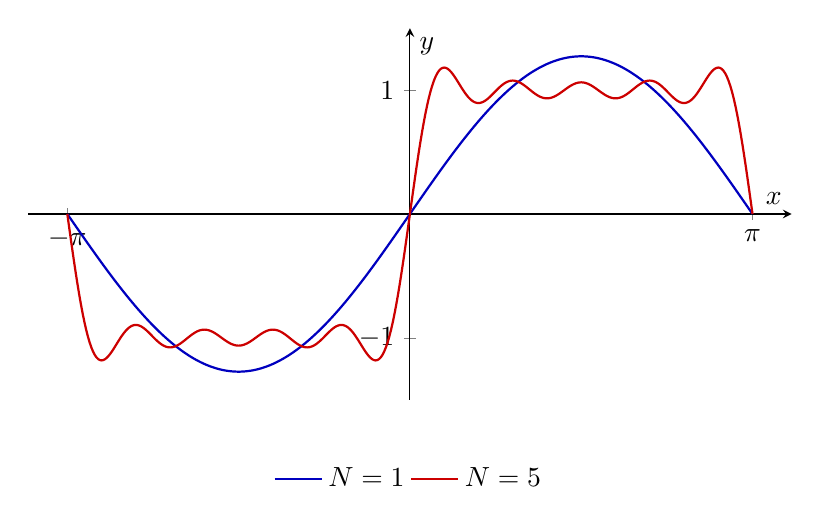
\begin{tikzpicture}
\begin{axis}[
  width=0.93\linewidth, height=6.3cm,
  axis lines=middle, xlabel={$x$}, ylabel={$y$},
  xmin=-3.5, xmax=3.5, ymin=-1.5, ymax=1.5,
  xtick={-3.14159265,0,3.14159265},
  xticklabels={$-\pi$,$0$,$\pi$}, ytick={-1,1},
  samples=401, domain=-pi:pi,
  legend style={at={(0.5,-0.15)}, anchor=north,
    draw=none, legend columns=2},
  every axis plot/.append style={thick}
]
\addplot[blue!75!black] {4/pi*sin(deg(x))};
\addlegendentry{$N=1$}
\addplot[red!80!black]
  {4/pi*(sin(deg(x))+sin(deg(3*x))/3+sin(deg(5*x))/5
        +sin(deg(7*x))/7+sin(deg(9*x))/9)};
\addlegendentry{$N=5$}
\end{axis}
\end{tikzpicture}
\caption{Partial sums \eqref{eq:partial} of the square wave.}\label{fig:square}
\end{figure}

Adding more terms improves the approximation away from the jumps,
as Figure~\ref{fig:square} shows.

\clearpage
\section{Convergence}\label{sec:convergence}
The following classical result tells where the series
\eqref{eq:series} converges, and to what.

\begin{theorem}[Dirichlet]\label{thm:dirichlet}
Let $f$ be $2\pi$-periodic and piecewise smooth in the sense of
Definition~\ref{def:piecewise}. Then the Fourier series
\eqref{eq:series} converges at every point $x$, and its sum is
\[
  \frac{f(x^{+})+f(x^{-})}{2}.
\]
In particular, the series converges to $f(x)$ wherever $f$ is continuous.
\end{theorem}

For the square wave of Section~\ref{sec:square}, the sum at $x=0$
is therefore $0$, the average of $-1$ and $1$.

\section{The Gibbs phenomenon}\label{sec:gibbs}
Near each discontinuity, a persistent overshoot remains:
the maximum of $S_N$ near $x=0$ tends to
\begin{equation}\label{eq:gibbs}
  \frac{2}{\pi}\int_0^{\pi}\frac{\sin t}{t}\,dt \approx 1.1790
\end{equation}
as $N\to\infty$. This is the \emph{Gibbs phenomenon}. It does not
contradict Theorem~\ref{thm:dirichlet}: at each fixed $x\neq0$ the
partial sums \eqref{eq:partial} still converge to $f(x)$, but the
place of the overshoot moves towards the jump.

\begin{theorem}\label{thm:mean}
For a square-integrable $f$, the partial sums of \eqref{eq:series}
converge to $f$ in the mean:
\[
  \lim_{N\to\infty}\int_{-\pi}^{\pi}\bigl|f(x)-S_N(x)\bigr|^2\,dx=0.
\]
\end{theorem}

Theorem~\ref{thm:mean} and the value \eqref{eq:gibbs} together show
that the overshoot of Figure~\ref{fig:square} occupies a smaller and
smaller interval, even though its height does not decrease.
\end{document}
